\chapter{Software and tools}

\section{Qt}
\todo[inline]{
\textbf{Todo}

- Short information about why Qt has been chosen

- Compiler version 

- OpenGL in qt
}

\section{OpenCV}

\todo[inline]{
\textbf{Todo}

- should I include this section even though it is not used in my project?
}

\section{GeoMod}

\todo[inline]{
\textbf{Todo}

- Move this to previous work?

- Who has created it and what is it's intention

- Feature set and main operation
}

\begin{figure}
 \centering 
 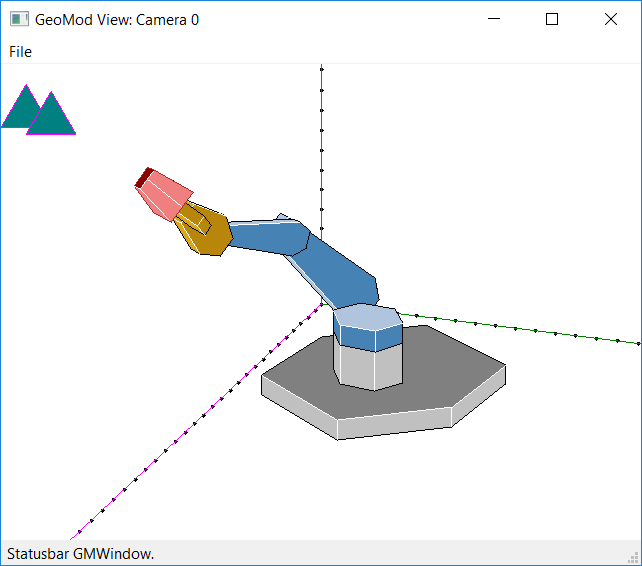
\includegraphics[width=.7\linewidth]{geomod_robot}
 \caption{GeoMod 3D visualization interface}
 \label{geomod_interface}
\end{figure}

\section{Representing time}\label{reptime}

A computer works in clock cycles and has no understanding of time. By counting the number of clock cycles and divide by clocks per second it is able to estimate the elapsed time. The \texttt{clock()} function contained in the standard c++ \texttt{time.h} library returns the total number of $ms$ elapsed since the program started. This has been used to calculate time-dependent animation and derivatives.
